%%%%%%%%%%%%%%%%%%%%%%%%%%%%%%%%%%%%%%%%%%%%%%%%%%%
%% LaTeX book template                           %%
%% Author:  Amber Jain (http://amberj.devio.us/) %%
%% License: ISC license                          %%
%%%%%%%%%%%%%%%%%%%%%%%%%%%%%%%%%%%%%%%%%%%%%%%%%%%

\documentclass[a4paper,11pt]{book}
\usepackage[T1]{fontenc}
\usepackage[utf8]{inputenc}
\usepackage{lmodern}
\usepackage{hyperref}
\usepackage{graphicx}
\usepackage[english]{babel}

% title and subtitle
\title{\Huge \textbf{Unified Heteregeneous Networking Middleware Project Report}  \\ 
\huge \vspace{5mm} Fall 2015 }
% Author
\author{\textsc{Jincheng Li}}

\begin{document}

\frontmatter
\maketitle

% Auto-generated table of contents, list of figures and list of tables %
\tableofcontents
\mainmatter

% NEW CHAPTER! %
\chapter{Introduction}
Devices with Internet access today are becoming increasingly mobile. The Heterogeneous Networking Middleware project provides a mechanism for devices to seamlessly handle network mobility, and make intelligent decisions about how and when to use different networks across multiple interfaces. \\
The prototype for this project started with a demo on Linux and is currently shifting to Android. Some work was done last semester to port the Linux implementation to Android, while this semester I took a different approach and re-implemented some of the necessary functionalities within the Android Java Frameork. \\
The project started in 2012 in the IRT lab. Over the course of one year 

\chapter{Architecture}

\chapter{Android Networking Stack}
In order to understand how Android performs network switching and the functionalities it provides similar to MIH, a fair amount of time was spent this semester researching the architecture of Android's networking stack. Here we present the details of our findings.

\section{Android Architecture}
Before we talk about the Android networking stack, we first introduce the architecture of the Android platform. Broadly speaking, Android consists of five layers: Linux kernel, HAL, Android runtime + native libraries, Android Framework, and user applications. These five layers are laid out in the following diagram: % elaborate...

% android architecture diagram here
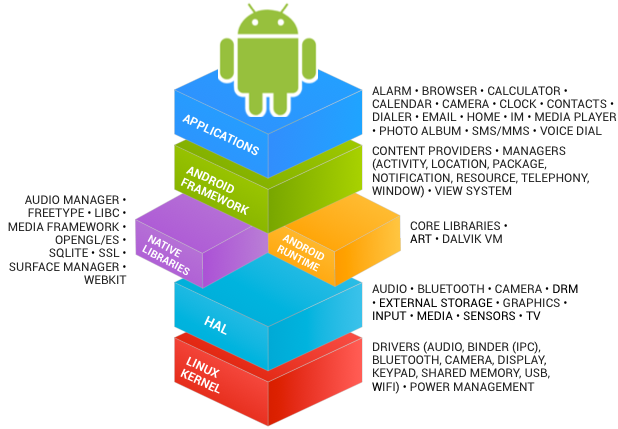
\includegraphics[width=\textwidth]{../android_framework_details.png}

At the bottom of the Android software stack is the Linux kernel, which provides a level of abstraction between the device hardware and the upper layers of Android. The kernel provides typical low-level system services such as process, memory management, and also includes essential device drivers for hardware such as cellular and WiFi NICs. \\
The hardware abstraction layer (HAL) defines a standard interface for hardware vendors to implement and allows Android to be agnostic about lower-level driver implementations. We don't discuss HAL at any more length here as it is not vital for our purposes. \\
Next comes the Android runtime (i.e. Davlik VM) and native libraries, which are implemented in C/C++. 

\section{General Networking}
The following classes deal with networking in general, regardless of the specific type of a network.

\subsection{ConnectivityManager}
In general, classes with a ``Manager'' suffix are singleton classes exposed as part of the Android API for applications. They serve as the interface between application developers and the Android framework. Methods in these classes do not usually contain intricate program logic, but simply call some other system service class (e.g. methods in ConnectivityManager call corresponding methods in ConnectivtyService) which actually implements the required functionality. \\
In the case of ConnectivityManager, it is reponsible for answering queries about the state of network connectivity, and for notifying applications about network connectivity changes. Additionally, it allows applications to request or select certain networks for their data traffic. This last feature is most relevant to our research. The method involved here is \verb|requestNetwork|, which takes as its input a \verb|NetworkRequest|, and a \verb|NetworkCallback|. 

\subsection{ConnectivityService}

\subsection{NetworkAgent and NetworkAgentInfo}

\section{WiFi Networks}

\subsection{WifiManager}
The WifiManager class is exposed as part of Android's application API. It provides methods for applications to manage all aspects of WiFi connectivity.

\subsection{WifiService}

\subsection{WifiStateMachine}

\subsection{WifiAutoJoinController}

\section{Cellular Networks}
\subsection{TelephonyManager}
\subsection{DataConnection}

\section{Another section heading}
Lorem ipsum dolor sit amet, consectetur adipisicing elit, sed do eiusmod tempor incididunt ut labore et dolore magna aliqua. Ut enim ad minim veniam, quis nostrud exercitation ullamco laboris nisi ut aliquip ex ea commodo consequat.

% Sample table                                        %
% Source: www1.maths.leeds.ac.uk/latex/TableHelp1.pdf %
\begin{table}[ht]
\caption{Sample table} % title of Table
\centering % used for centering table
\begin{tabular}{c c c c}
% centered columns (4 columns)
\hline\hline %inserts double horizontal lines
S. No. & Column\#1 & Column\#2 & Column\#3 \\ [0.5ex]
% inserts table
% heading
\hline % inserts single horizontal line
1 & 50 & 837 & 970 \\
2 & 47 & 877 & 230 \\
3 & 31 & 25 & 415 \\
4 & 35 & 144 & 2356 \\
5 & 45 & 300 & 556 \\ [1ex] % [1ex] adds vertical space
\hline %inserts single line
\end{tabular}
\label{table:nonlin} % is used to refer this table in the text
\end{table}

Duis aute irure dolor in reprehenderit in voluptate velit esse cillum dolore eu fugiat nulla pariatur. Excepteur sint occaecat cupidatat non proident, sunt in culpa qui officia deserunt mollit anim id est laborum. \\ Lorem ipsum list:
\begin{itemize}
\item Mauris sit amet nulla mi, vitae rutrum ante.
\item Maecenas quis nulla risus, vel tincidunt ligula.
\item Nullam ac enim neque, non \emph{dapibus} mauris.
\end{itemize}

\noindent Lorem ipsum dolor sit amet, consectetur adipiscing elit. Duis risus ante, auctor et pulvinar non, posuere ac lacus. Praesent egestas nisi id metus rhoncus ac lobortis sem hendrerit. Etiam et sapien eget lectus interdum posuere sit amet ac urna\footnote{Lorem ipsum dolor sit amet, consectetur adipiscing elit. Duis risus ante, auctor et pulvinar non, posuere ac lacus.}:

\subsection{Lorem ipsum dolor sit amet, consectetur adipiscing elit.}
Lorem ipsum dolor sit amet, consectetur adipiscing elit. Duis risus ante, auctor et pulvinar non, posuere ac lacus. Praesent egestas nisi id metus rhoncus ac lobortis sem hendrerit. Etiam et sapien eget lectus interdum posuere sit amet ac urna. Aliquam pellentesque imperdiet erat, eget consectetur felis malesuada quis. Pellentesque sollicitudin, odio sed dapibus eleifend, magna sem luctus turpis, id aliquam felis dolor eu diam. Etiam ullamcorper, nunc a accumsan adipiscing, turpis odio bibendum erat, id convallis magna eros nec metus. Sed vel ligula justo, sit amet vestibulum dolor. Sed vitae augue sit amet magna ullamcorper suscipit. Quisque dictum ipsum a sapien egestas facilisis. 

\subsection{Lorem ipsum dolor sit amet, consectetur adipiscing}
Lorem ipsum dolor sit amet, consectetur adipiscing elit. Duis risus ante, auctor et pulvinar non, posuere ac lacus. Praesent egestas nisi id metus rhoncus ac lobortis sem hendrerit. Etiam et sapien eget lectus interdum posuere sit amet ac urna. Aliquam pellentesque imperdiet erat, eget consectetur felis malesuada quis. Pellentesque sollicitudin, odio sed dapibus eleifend, magna sem luctus turpis, id aliquam felis dolor eu diam.

\end{document}
